\begin{figure}[h]
    \centering
    \caption{Desempenho da solução 4\_tom para diferentes valores de refinamento da função custo, parâmetro C do classificador SVC.}
    % \vspace{-0.5cm}
    \begin{subfigure}{.5\textwidth}
        \centering
        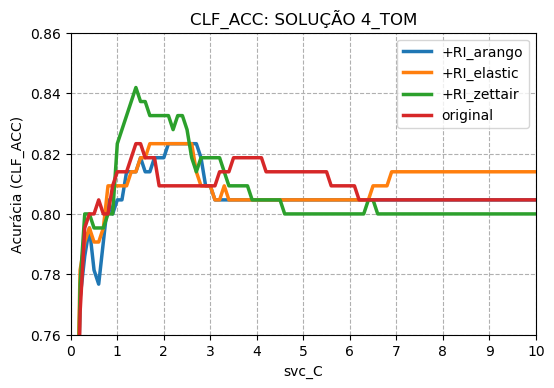
\includegraphics[width=\textwidth]{img/clf-acc-4-tom.png}
        \caption{CLF\_ACC}
        \label{fig:clf-acc-4-tom}
    \end{subfigure}%
    \begin{subfigure}{.5\textwidth}
        \centering
        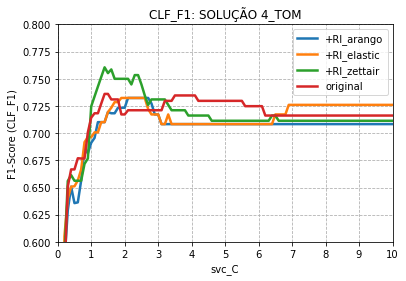
\includegraphics[width=\textwidth]{img/clf-f1-4-tom.png}
        % \includegraphics[width=.4\linewidth]{image1}
        \caption{CLF\_F1}
        \label{fig:clf-f1-4-tom}
    \end{subfigure}
    % \begin{center}
    %     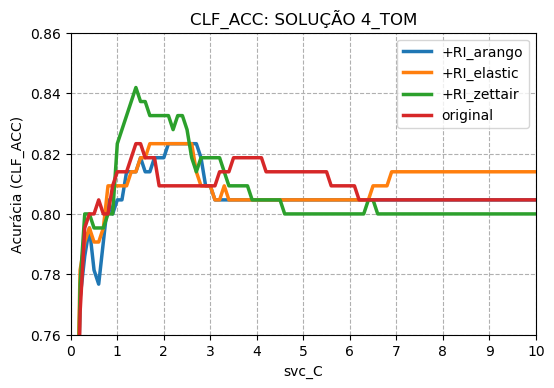
\includegraphics[scale=0.75]{img/clf-acc-4-tom.png}
    % \end{center}
    \vspace{-0.5cm}
    \legend{\ABNTEXfontereduzida \textbf{Fonte:} O autor.}
    \label{fig:clf-4-tom}
\end{figure}